\documentclass{beamer}
% Use option "handout" here to collapse multi-page slides built from
% \uncover or \pause commands.
%\documentclass[handout]{beamer}

\usetheme{Antibes}
\usecolortheme{lily}

\mode<presentation>

\title[Abbrv. Title]{Long Complex Title}
\author{Your Name \\ \texttt{contact@email.address}}
\date{11 January 2012}

\begin{document}

% =============================================================================
% Front slide.
{
  \usebackgroundtemplate{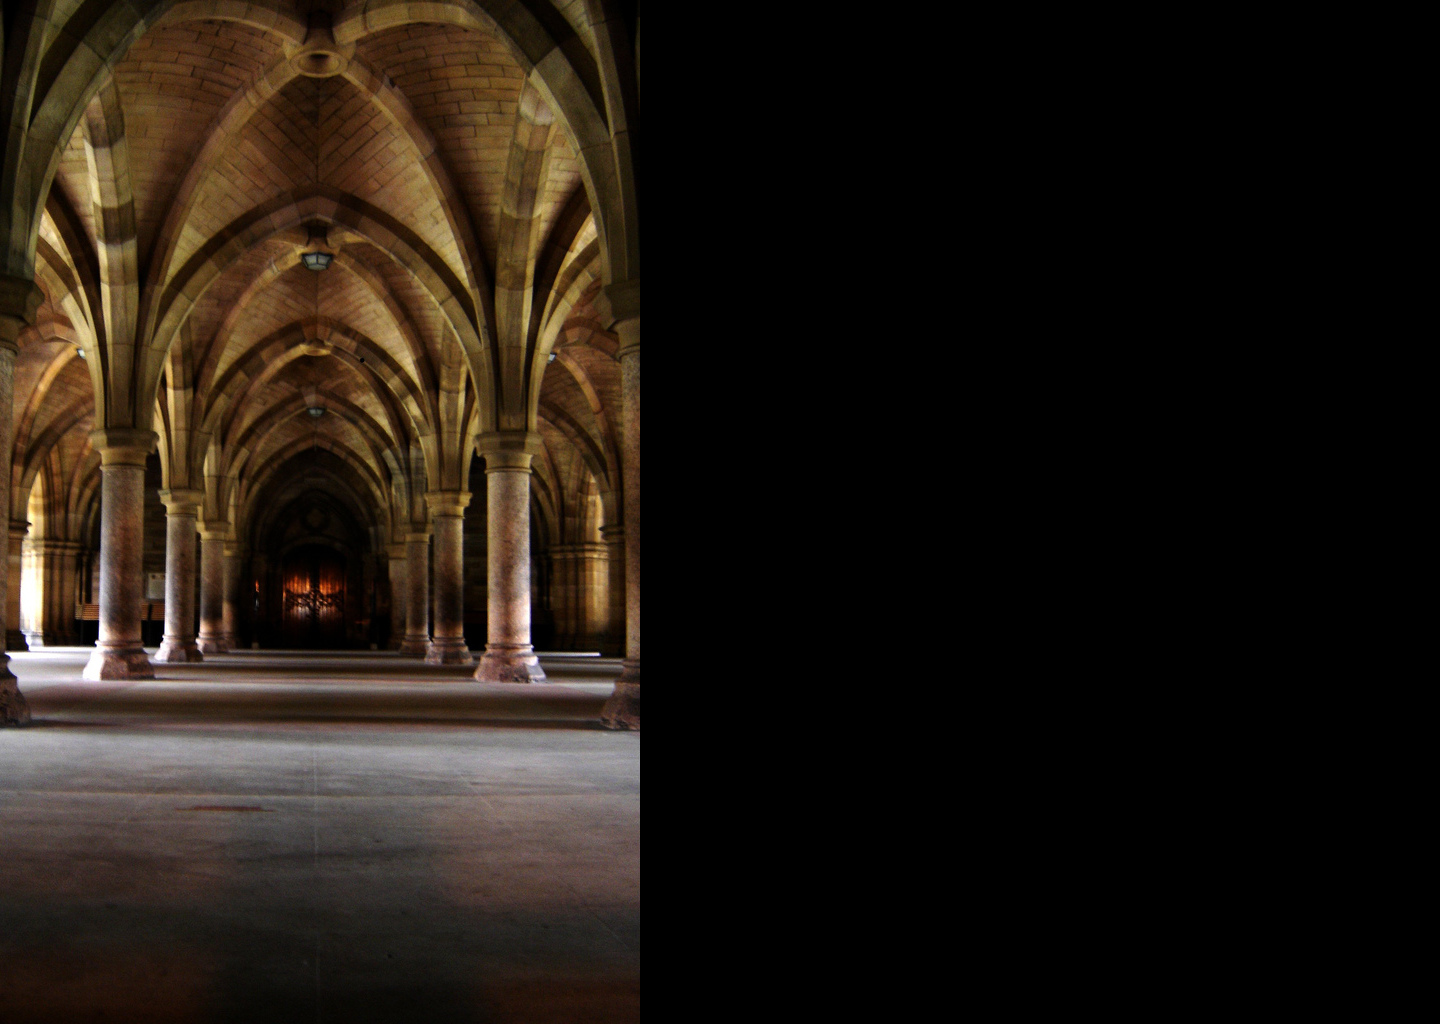
\includegraphics[height=\paperheight]{cloisters}}

  \begin{frame}[plain]
    \setbeamercolor{title}{fg=white}
    \setbeamercolor{author}{fg=white}
    \setbeamercolor{date}{fg=white}

    \begin{columns}

      \begin{column}[l]{5cm}
      \end{column}

      \begin{column}[r]{5cm}
        \titlepage
      \end{column}

    \end{columns}
  \end{frame}
}

% Table of contents.
\begin{frame}
\frametitle{Outline}
\tableofcontents
\end{frame}

% =============================================================================
\section{The Start of an Awesome Talk}

% -----------------------------------------------------------------------------
\begin{frame}
\frametitle{Outline}
\tableofcontents[currentsection]
\end{frame}

% -----------------------------------------------------------------------------
\begin{frame}

  Here, I'm going to enumerate a bunch of cool things.

  \begin{enumerate}

    \pause
  \item Cool thing!

    \pause
  \item Another cool thing!

  \end{enumerate}

\end{frame}


% -----------------------------------------------------------------------------
\begin{frame}

  Here's another ace slide in the same section!

\end{frame}


% =============================================================================
\section{The End of an Awesome Talk}

% -----------------------------------------------------------------------------
\begin{frame}
\frametitle{Outline}
\tableofcontents[currentsection]
\end{frame}


% -----------------------------------------------------------------------------
\begin{frame}

  Great talk!

  \begin{itemize}
  \item \uncover<2->{Key point 1!}
  \item \uncover<3->{Key point 2!}
  \item \uncover<4->{Key point 3!}
  \end{itemize}

\end{frame}


% =============================================================================
% Back slide.
{
  \usebackgroundtemplate{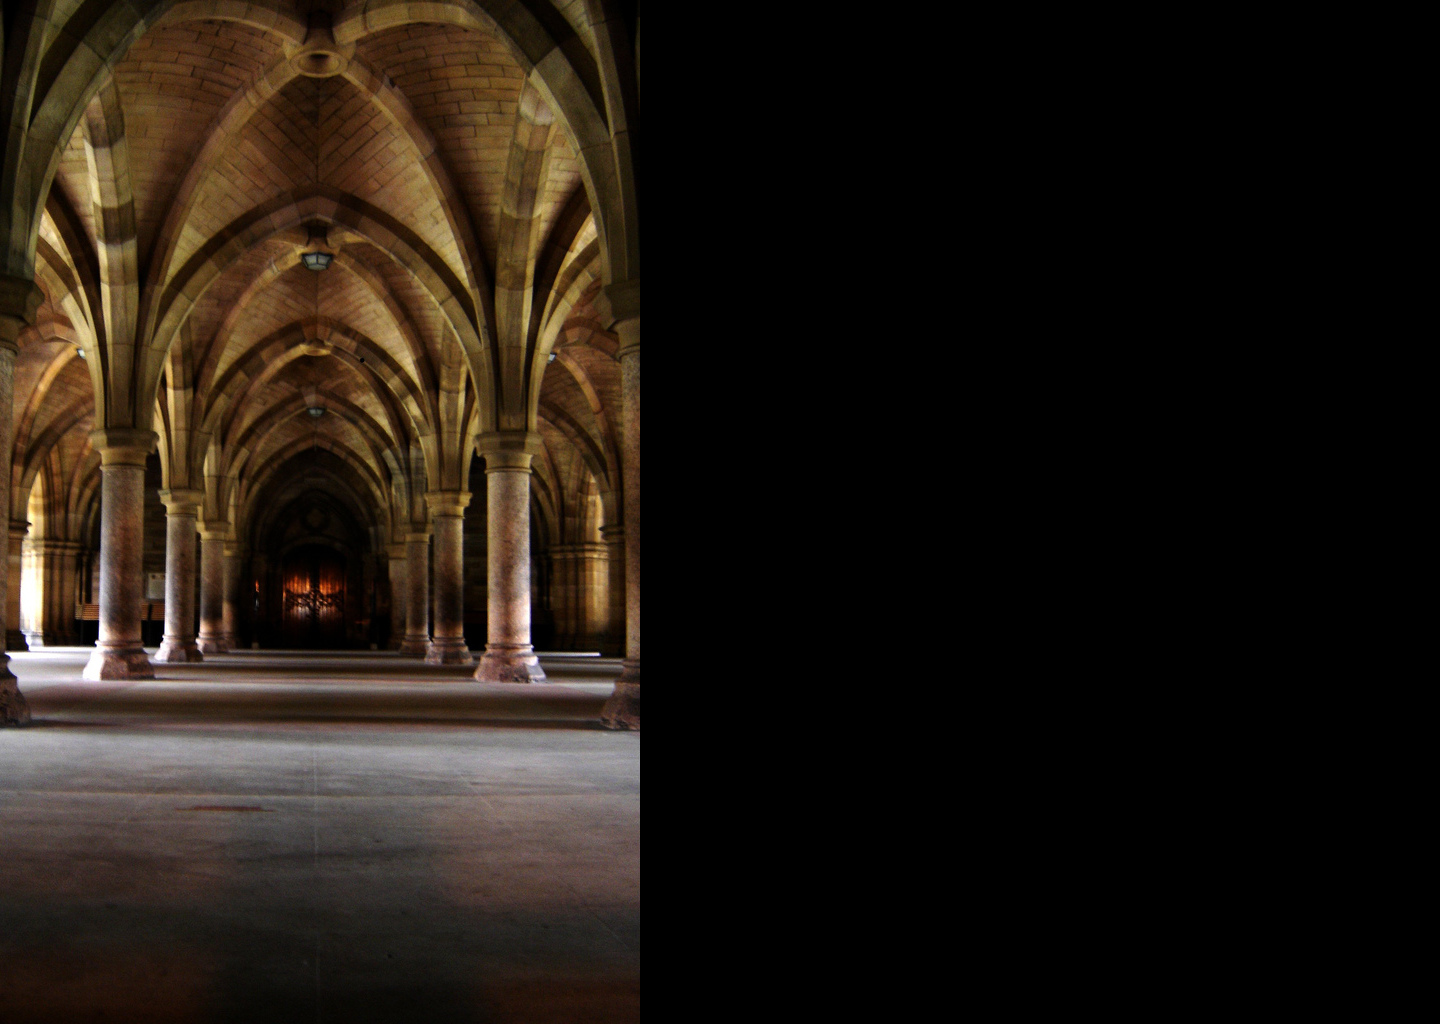
\includegraphics[height=\paperheight]{cloisters}}

  \begin{frame}[plain]

    \begin{columns}

      \begin{column}[l]{5cm}
      \end{column}

      \begin{column}[r]{5cm}
        \textcolor{white}{
          Questions?
        }
      \end{column}

    \end{columns}
  \end{frame}
}


\end{document}
